\chapter{Planung}\label{Planung}
Bevor mit der Umsetzung begonnen wird, muss geklärt werden, welche Schritte notwendig sind und in welcher Reihenfolge sie sinnvoll sind. Die Planung schafft die Grundlage , auf der die spätere Umsetzung aufsetzt, um eine reibungslosere Entwicklung zu ermöglichen.

%Harm
%Passt
\section{Zeitplanung}\label{Zeitplanung}
Zuerst müssen Informationen über das Themengebiet gesammelt werden. Danach erfolgt der
Entwurf eines Konzepts mit anschließender Technologieauswahl. Nachdem die
Technologieauswahl getroffen ist, wird die notwendige Hardware beschafft und
parallel dazu mit der Aufteilung der Aufgaben in Arbeitspakete begonnen. Im
nächsten Schritt werden die Arbeitspakete in logischer Abfolge abgearbeitet und
das Konzept so schrittweise umgesetzt.\\
Die Zeitplanung ist semesterbedingt in zwei große Blöcke unterteilt.\\
Im ersten Semester werden folgende Punkte umgesetzt:

\begin{enumerate}
	\item Informationsbeschaffung
	\item Entwicklung eines Konzeptes
	\item Technologieauswahl
	\item Beschaffung von notwendiger Hard- und Software
	\item Aufteilung der Aufgaben in Arbeitspakete
	\item Erstellen der Zeitplanung
\end{enumerate}

Im zweiten Semester werden folgende Punkte umgesetzt:

\begin{enumerate}
	\item Abarbeitung der Arbeitspakete
	\item Erstellung der Dokumentation
\end{enumerate}
%Jan
%Passt
\subsection{GANTT-Diagramm}
Die genannten Punkte im \fullref{Zeitplanung} müssen zeitlich strukturiert in einem GANTT-Diagramm festgehalten werden.
Die folgenden GANTT-Diagramme wurden für die zwei Phasen im Rahmen der Zeitplanung erstellt:
\begin{landscape}
	\begin{figure}[htb]
		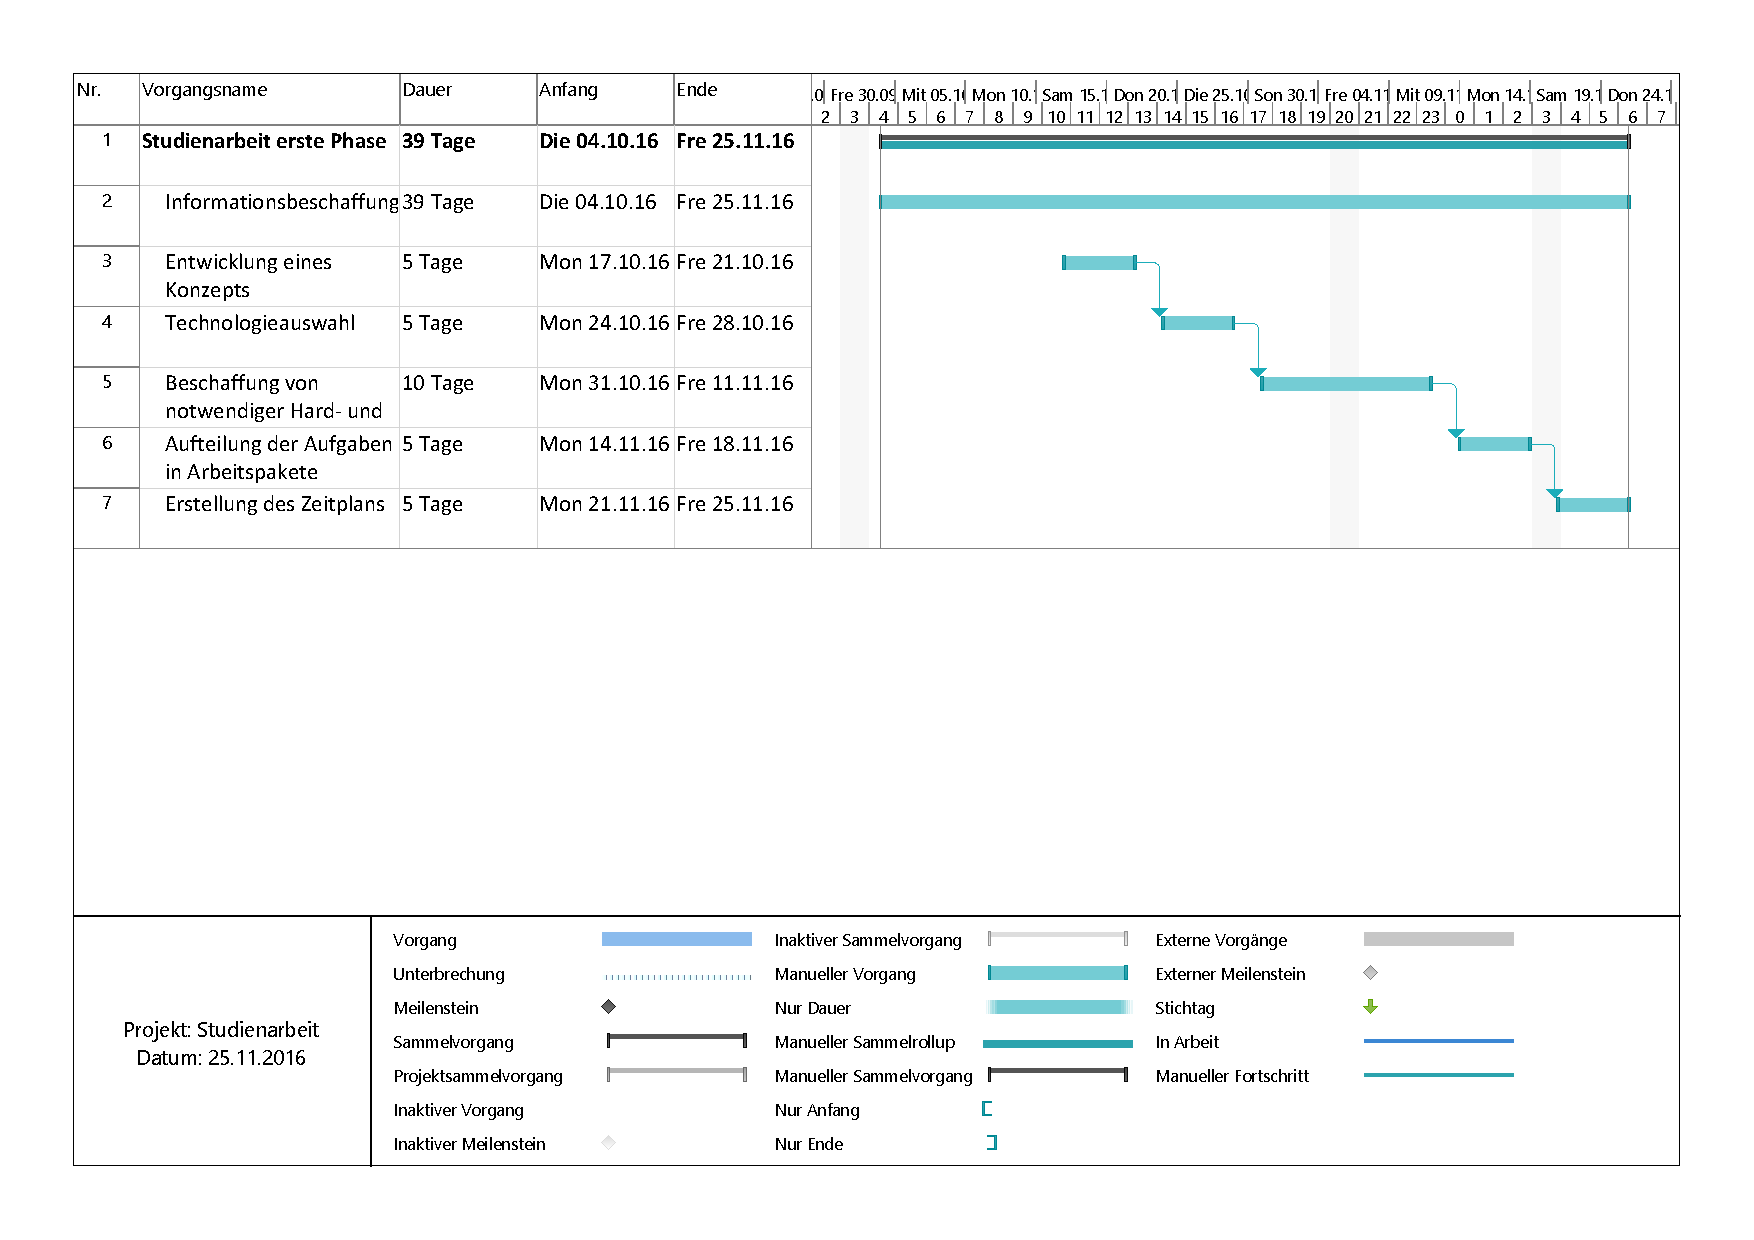
\includegraphics[width=\linewidth, height=.9\textheight]{Bilder/GANTT/Studienarbeit_erste_Phase.pdf}
		\caption[GANTT-Diagramm: Studienarbeit erste Phase]{Studienarbeit erste Phase}
		\label{fig:Studienarbeit_erste_Phase}
	\end{figure}
\end{landscape}
\begin{landscape}
	\begin{figure}[htb]
		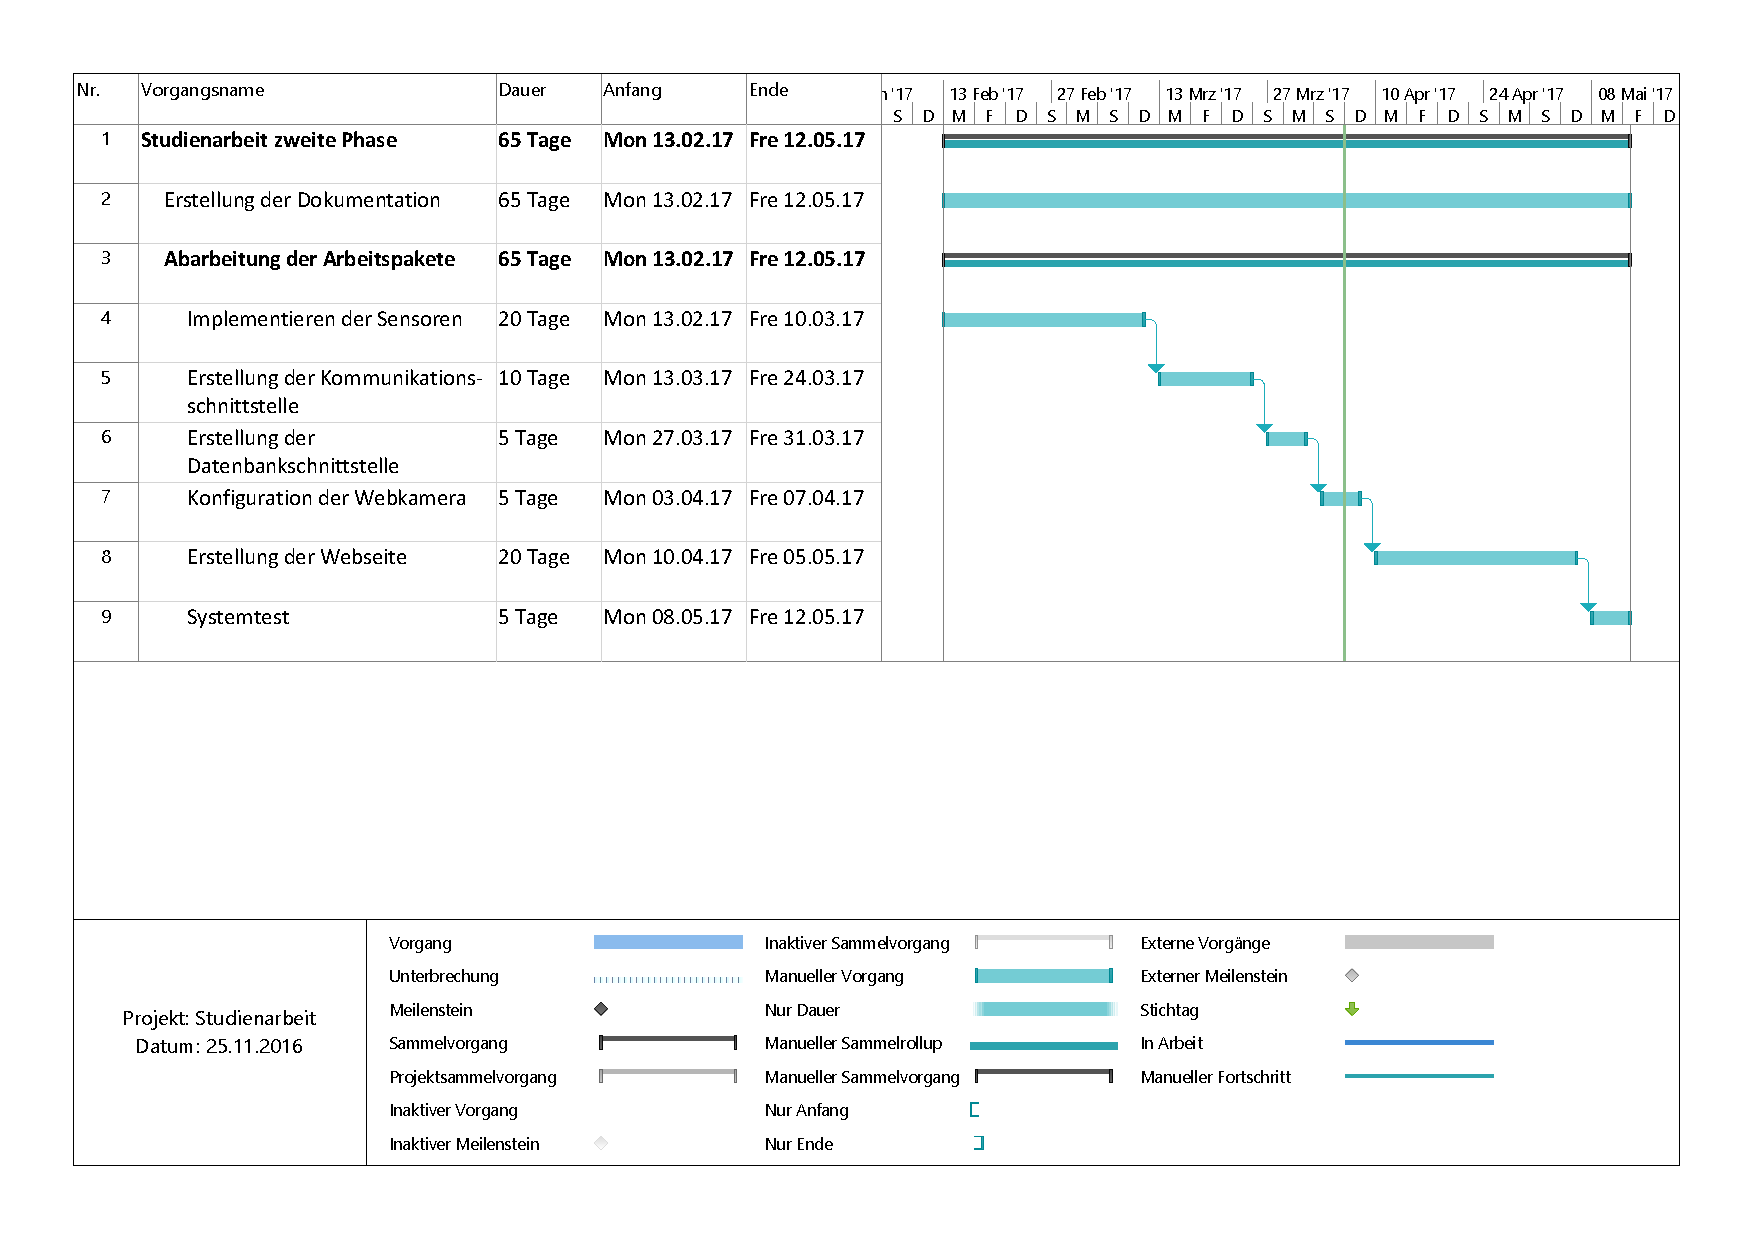
\includegraphics[width=\linewidth, height=.9\textheight]{Bilder/GANTT/Studienarbeit_zweite_Phase.pdf}
		\caption[GANTT-Diagramm: Studienarbeit zweite Phase]{Studienarbeit zweite Phase}
		\label{fig:Studienarbeit_zweite_Phase}
	\end{figure}
\end{landscape}

%Passt
\section{Netzwerkplanung}
Eine zentrale Funktionalität ist die Datenübertragung, weshalb das Netzwerk eine besonders kritische Komponente ist. Das Netzwerk ist eine der ersten Komponenten, die funktionieren muss, damit beim späteren entwickeln auf eine funktionierende Infrastruktur zurückgegriffen werden kann.

%Harm
\subsection{Netzwerkplan}
Der Netzwerkplan soll schematisch darstellen, wie das Netzwerk funktioniert. Er gibt einen Überblick über die beteiligten Komponenten und illustriert schematisch wie die Verbindungen aussehen.\\
Die Sensoren sind an den jeweiligen Sensorknoten angeschlossen. Die Daten werden per WLAN an die Zentraleinheit gesendet. Dort werden die Daten in die Datenbank
geschrieben.\\
Der Webserver greift auf die Datenbank zu und stellt die Daten auf einer Webseite
übersichtlich dar. (\fullref{Darstellung_Umgebung})
%TODO: Feinschliff Netzplan - Nachfragen was gemacht werden soll
	%TODO: PC's durch kleine Rasbpis ersetzt werden (Visio vorlagen)
\begin{figure} [htb]
\begin{centering}
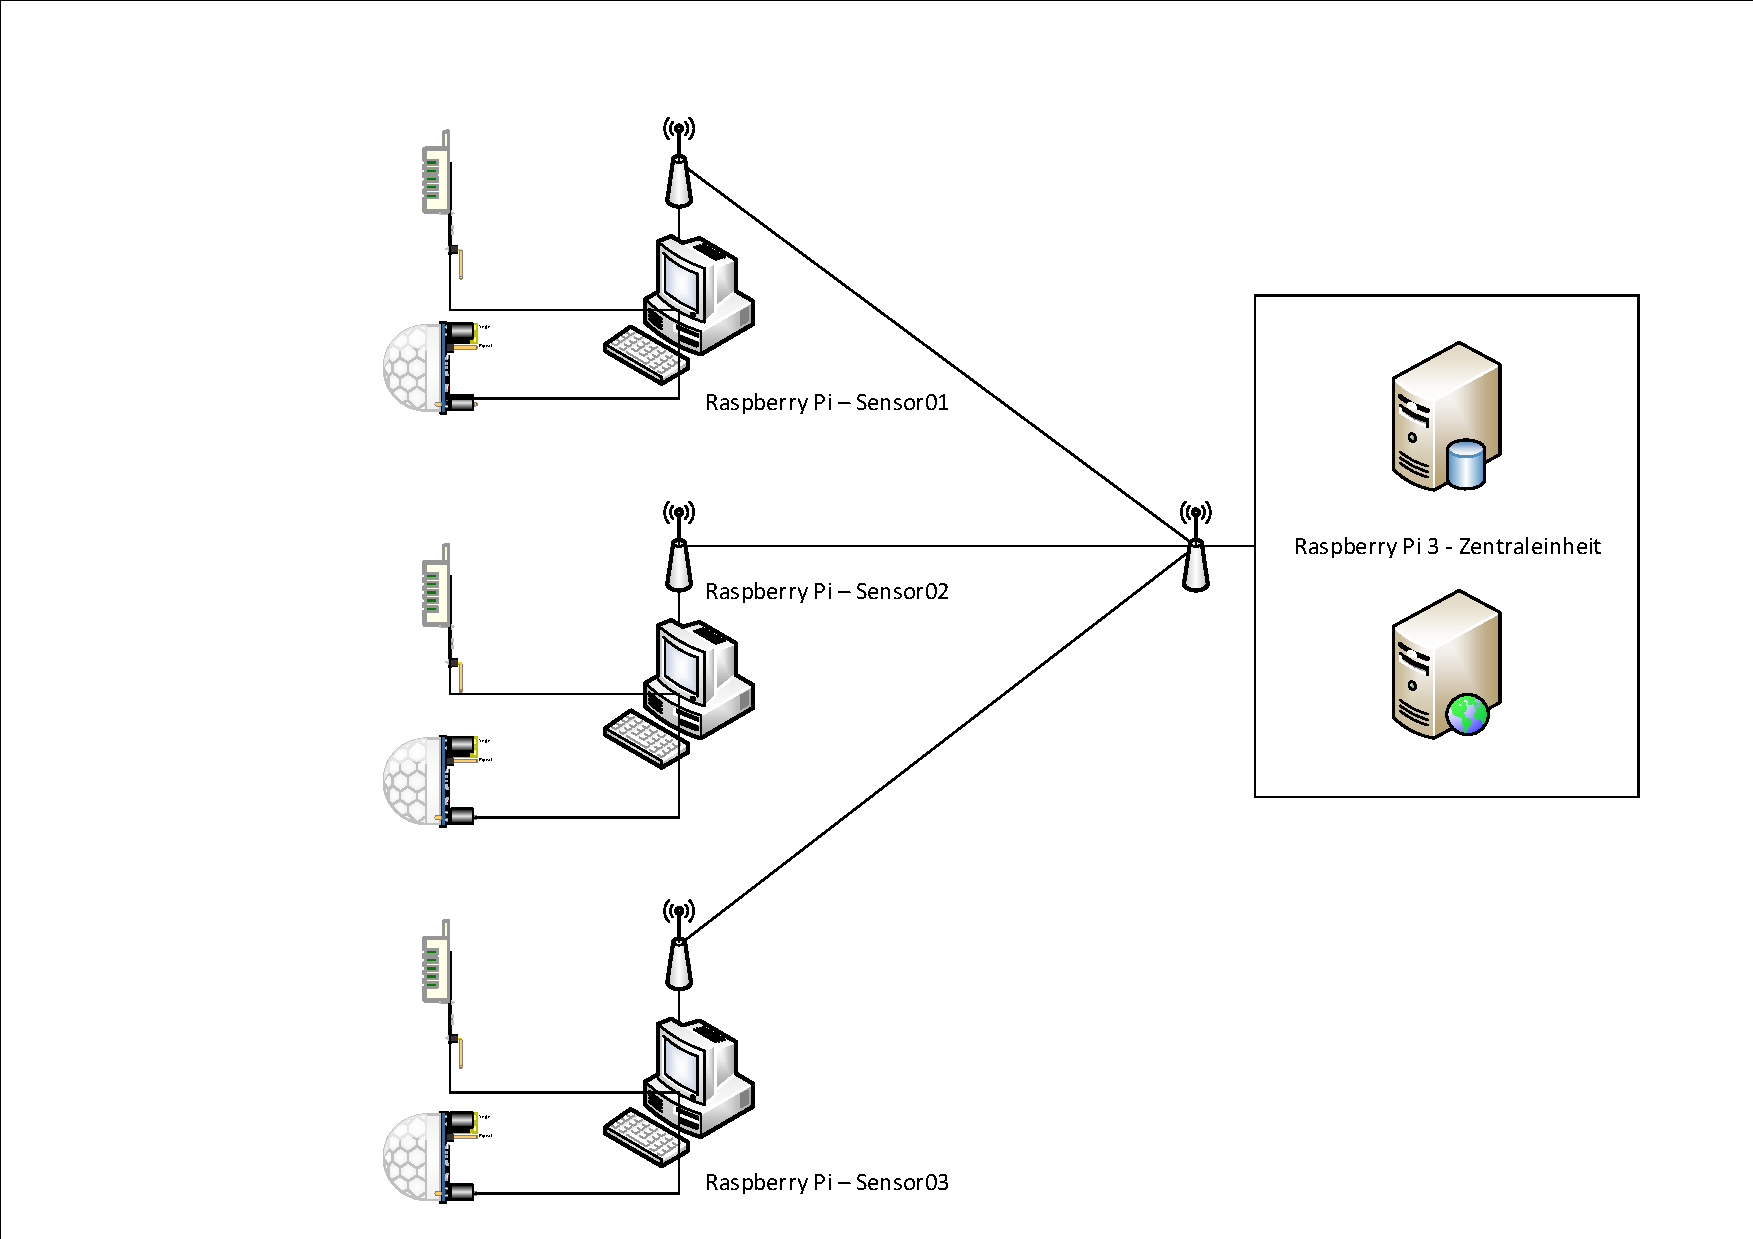
\includegraphics[scale=0.4]{Bilder/Kapitel3/Netzplan.pdf}
\caption[Schematische Darstellung der geplanten Umgebung]{Schematische
Darstellung der geplanten Umgebung}
\label{Darstellung_Umgebung}
\end{centering}
\end{figure} 

%Harm
%Passt
\subsection{Kommunikation}
Die Kommunikation soll auf IP-Adressen und TCP-Sockets in einem WLAN-Funknetz basieren. Ein Sensorknoten soll über den \ac{DHCP}-Server eine IP-Adresse erhalten. Die IP-Adresse ist notwendig, damit der Sensorknoten einen Socket öffnen kann und die Daten an die Zentraleinheit absenden kann. 

%Alex
%Passt
\section{Sensorknoten}
%TODO: Erwähnen, dass mehrere Sensorknoten geben kann
Ein Raspberry Pi, an dem die Messdaten der Sensoren gesammelt werden, wird als Sensorknoten bezeichnet. An diesen können bis zu sieben Sensoren, die im \fullref{Sensoren_Planung} beschrieben sind, angeschlossen werden. Neben dem Messen muss der Sensorknoten die Messdaten an die Zentraleinheit weiterleiten, welche die Daten auswertet. Bevor der Sensorknoten implementiert werden kann, muss eine Auswahl der Programmiersprache getroffen werden.

%Jan
\subsection{Python vs. Java}
Für das Projekt ist die richtige Programmiersprache essenziell. Die Sprache muss nicht nur die Daten der Sensoren auslesen, sondern diese auch in Pakete packen und an die Zentraleinheit weitergeben. Die Weitergabe der Datenpakete soll über einen TCP-Socket erfolgen, welcher von der ausgewählten Sprache erstellt werden können muss. Hierzu werden zwei Programmiersprachen verglichen, Java (siehe \fullref{Java}) und Python (siehe \fullref{Python}). Folgende Tabelle vergleicht die Funktionalitäten der Sprachen, die für das Projekt notwendig sind:\hfill

\begin{table}[htb]
	\centering
	\caption{Python vs. Java}
	\label{tab:phytionvsjava}
	\begin{tabular}{l|l|l}
	\textbf{Funktionalität} & \textbf{Java} &\textbf{Python}   \\
	\hline
	 Speicherverbrauch & hoch & niedrig \\\hline
	Komplexität  & hoch & niedrig\\\hline
	Geschwindigkeit  & hoch & hoch \\\hline
	Bibliotheken für die Sensoren & nicht vorhanden & vorhanden \\\hline
	Schnittstelle für die Datenübertragung & vorhanden & vorhanden
	\end{tabular}
\end{table}
\noindent Da die Raspberry Pi's für schnelle, kleine und hardwarenahe Projekte ausgelegt sind, fiel die Entscheidung auf die Sprache Python. Da Java nur bedingt hardwarenah ist und die Speicherkapazität der Raspberry Pi's begrenzt ist. Ein weiterer Vorteil von Python sind die bereits vorhandenen Bibliotheken und die kurze Einarbeitungszeit. Die kürzere Einarbeitungs- und Umsetzungszeit, kommt der engmaschigen \nameref{Zeitplanung} (siehe \fullref{Zeitplanung}) zugute.

%Alex
\subsection{Auslesen der Sensoren}
%TODO: Priorisierung der Sensoren
%TODO: Allgemeine Messdatenformat
%Jan
%Passt
\section{Zentraleinheit}
Die Zentraleinheit soll dafür zuständig sein, die ausgelesenen Daten der Sensorknoten, die im \fullref{Sensoren_Planung} beschrieben sind, in einer Datenbank zu speichern. Dazu wird eine Schnittstelle benötigt, welche die gesendeten Sensordaten der jeweiligen Sensorknoten annimmt, verarbeitet und in der Datenbank ablegt. Zusätzlich soll auf der Zentraleinheit eine Webseite entstehen, welche die zuvor gesammelten Daten aus der Datenbank ausliest und diese auf der Webseite möglichst zeitnah anzeigt.

%Jan
%Passt
\subsection{Datenbank}\label{sub:Datenbank}
Damit die Daten strukturiert gesammelt werden können, muss ein Datenbankentwurf gemacht werden. Dieser soll schematisch zeigen wie die Datenbank aufgebaut und die Daten abgespeichert werden sollen. Der Datenbankentwurf sieht wie folgt aus:
%TODO: Datenbankentwurf überarbeiten und horizontal zentrieren
\begin{landscape}
	\begin{figure}[ht]
		\begin{center}
			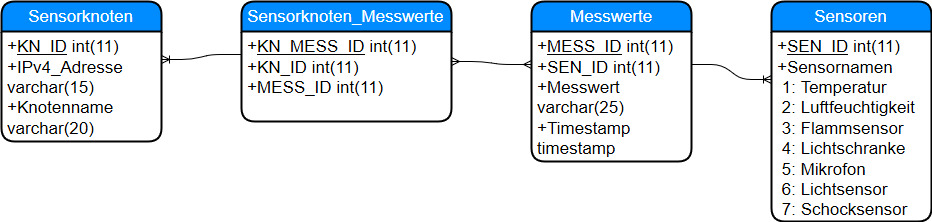
\includegraphics[width=\paperwidth]{Bilder/Kapitel3/Datenbankentwurf1.jpg}
			\caption[Schematische Darstellung des Datenbankentwurfs]{Schematische Darstellung des Datenbankentwurfs}
			\label{fig:Datenbankentwurf}
		\end{center}
	\end{figure}
\end{landscape}
\begin{description}
	\item[Tabelle Sensorknoten] \hfill \\
		In der Tabelle Sensorknoten sollen alle im Netzwerk befindlichen Sensorknoten abgelegt werden. Die Sensorknoten werden mit ihrem Knotennamen und ihrer IP-Adresse abgespeichert.
	\item[Tabelle Sensorknoten\_Messwerte] \hfill \\
		Die Tabelle Sensorknoten\_Messwerte soll als Hilftabelle dienen und den Sensorknoten ihre Messwerte zuordenen. Dies soll über die Fremdschlüssel KN\_ID und Mess\_ID geschehen.
	\item[Tabelle Messwerte] \hfill \\
		In der Tabelle Messwerte sollen die Messwerte der Sensorknoten in das Attribut Messwerte gespeichert werden. Damit erkennbar ist, welchem Sensor der Messwert zuzuordnen ist, soll die SEN\_ID als Fremdschlüssel zeigen, um welchen Sensor es sich handelt. Zusätzlich soll ein Attribut Timestamp der Tabelle hinzugefügt werden. Hier soll der jeweilige Zeitstempel beim Erzeugen des Eintrags hinterlegt werden.
	\item[Tabelle Sensoren] \hfill \\	
		Die Tabelle Sensoren, soll alle Sensoren beinhalten, die an die jeweiligen Sensorknoten angeschlossen werden können. Die Sensoren sollen mit einer festen SEN\_ID und einem festen Namen versehen werden.
\end{description}

%Harm
%Passt
\subsection{Webseite}\label{sub:Webseite}

Auf der Webseite soll sich ein Benutzer einloggen oder registrieren können.
Nach dem Login soll der Benutzer zu einer Übersicht weitergeleitet werden, auf der alle Sensorknoten in Tabellenform mit den aktuell gemessenen Werten abgebildet sind. \\
Auf einer Statistik-Seite soll ein Verlauf über mehrere Tage zu einem Sensor sichtbar sein.\\
Eine Webcam-Seite soll dazu dienen, auf eine angeschlossene Webcam zuzugreifen.\\
Ein Impressum soll eine kurze Information anzeigen, wer dieses Projekt umgesetzt hat.\\
Auf einer Logout-Seite soll der Benutzer die Meldung sehen, dass er ausgeloggt ist und eine Möglichkeit angeboten bekommen, um zurück zur Login-Seite zu gelangen.
(\fullref{Darstellung_Website_einfach})

\begin{figure} [htb]
\begin{centering}
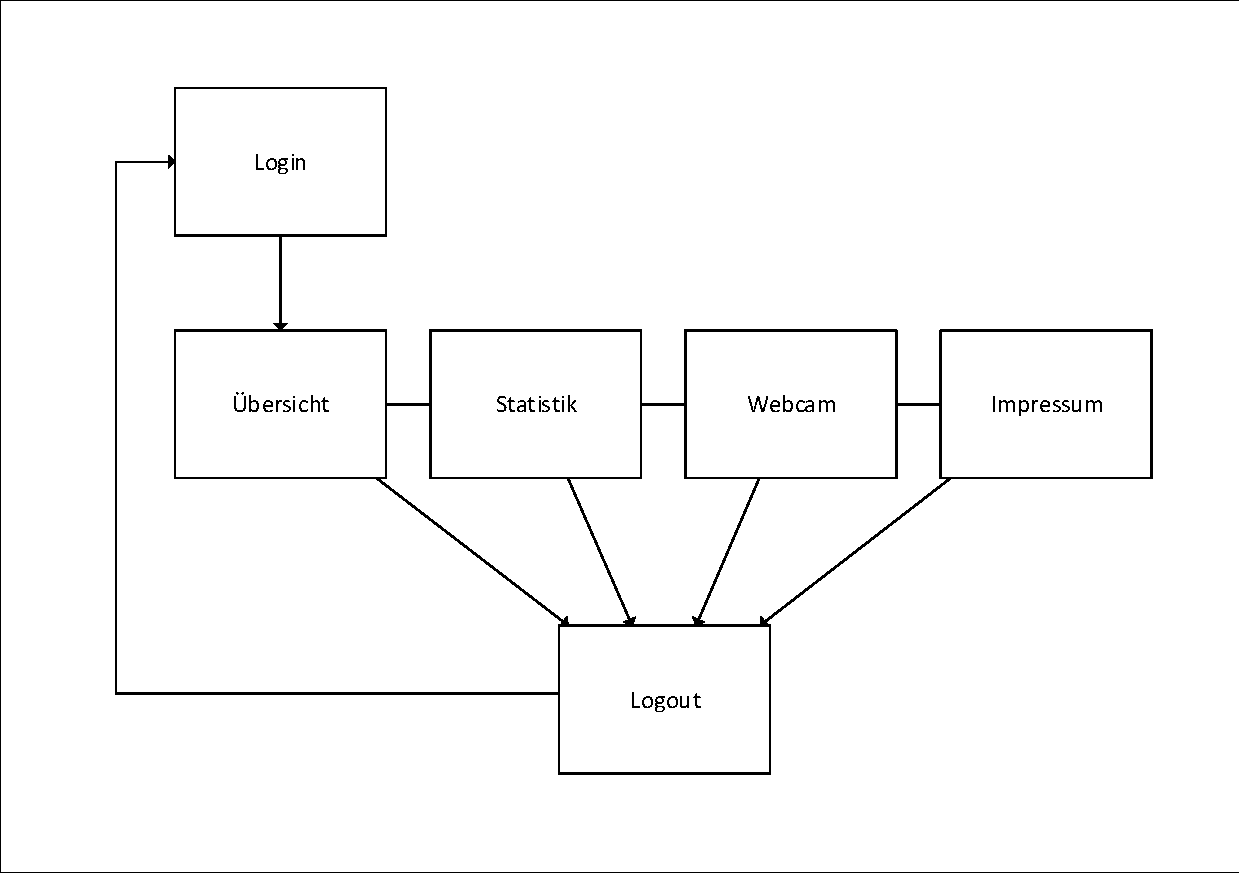
\includegraphics[scale=0.8]{Bilder/Kapitel3/struktur_website_einfach.pdf}
\caption[Schematische Darstellung der geplanten Webseite]{Schematische
Darstellung der geplanten Webseite}
\label{Darstellung_Website_einfach}
\end{centering}
\end{figure}

%Alle
%Passt
\section{Planungsresultat}

Die Sensoren sollen kontinuierlich abgefragt werden und senden die gemessenen Werte an
die Datenbank auf der Zentraleinheit. Dort sollen die Daten entsprechend dem
meldenden Sensorknoten abgespeichert werden. Die Website greift auf die Datenbank zu
und lädt die Daten in eine tabellarische Darstellung, die dem Benutzer angezeigt wird. Durch einen Zeitstempel ist es möglich bei Daten der Temperatursensoren
und der Feuchtigkeitssensoren einen Verlauf darzustellen.
